\documentclass{standalone}
\usepackage{tikz}

%x step={
\usetikzlibrary{decorations.pathmorphing}
%x }

\begin{document}

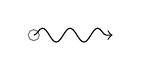
\begin{tikzpicture}
%x description="draw a line with a corner using absolute coordinates"
\draw[gray] (0,0) circle[radius=2pt];
%x step={
	\draw 
		[->, decorate,decoration=snake]
		(0,0) -- (1,0);
%x }
\end{tikzpicture}

\end{document}
